\documentclass[fontsize=14pt]{scrreport}
\usepackage{amssymb}
\usepackage[english,russian]{babel}
\usepackage{tikz}
\usepackage{setspace}
\linespread{1.3}
\usepackage{xcolor}
\usepackage{hyperref}
\usepackage{multirow,tabularx}
\newcolumntype{Y}{>{\centering\arraybackslash}X}
\renewcommand{\arraystretch}{1.3}
\usepackage[nottoc,notlof,notlot]{tocbibind} 
\usepackage{comment}
\usepackage{geometry}
\usepackage{amsmath}
\usepackage{graphicx}
\usepackage{nomencl}
\usepackage{fancyhdr}
\usepackage{caption}
\usepackage{float}
\floatstyle{plaintop}
\restylefloat{table}
\usepackage[tableposition=top]{caption}
\usepackage{subcaption}
\usepackage{hyperref}
\usepackage{comment}
\renewcommand{\thechapter}{\arabic{chapter}}
\def\bibname{Литература}
\makeatletter
\renewcommand{\@biblabel}[1]{#1.}
\makeatother

\graphicspath{{pictures/}}
\DeclareGraphicsExtensions{.pdf,.png,.jpg}
\linespread{1.6}
\geometry{
	paper=a4paper,
	top=2.5cm,
	bottom=2.5cm,
	right=2.5cm,
	left=3.5cm
}
\begin{document}
	\begin{titlepage}
		\begin{center}РЕСПУБЛИКА УЗБЕКИСТАН
 	МИНИСТЕРСТВО ВЫСШЕГО И СРЕДНЕГО-СПЕЦИАЛЬНОГО ОБРАЗОВАНИЯ \\ 
 	НАЦИОНАЛЬНЫЙ  УНИВЕРСИТЕТ УЗБЕКИСТАНА\\ИМЕНИ МИРЗО УЛУГБЕКА\\
	\begin{flushright}
			\small{На правах рукописи}\\
           \small{ УДК  539.172.12    }
			\end{flushright}
			\vfill

\textrm{Ашуров Синдоржон Ахмаджон угли}	\\		
			\large \textbf{Исследование развал ядра кислорода на $\alpha$-частицу и $^{12}$C в $^{16}$Оp соударениях при 3,25 А ГэВ/с }
			
		\end{center}
\begin{center}
5A140207 -- Ядерная физика и ядерные технологии (по областям применения)
\end{center}
         \vfill
         \begin{center}
         \textbf{ДИССЕРТАЦИЯ}\\
         на соискание степени\\
         Магистра
         \end{center}
         
         \begin{flushright}
Научный руководитель:\\
д.ф.-м.н, проф. БОЗОРОВ Э.Х.
         \end{flushright}
		\vfill
		\vfill
		\begin{center}
			г. Ташкент-2021
		\end{center}
	\end{titlepage}
	\newpage
	\renewcommand{\figurename}{Рисунок}
	\makenomenclature 
	\renewcommand{\nomname}{Список сокращений}
    \newcommand*{\nom}[2]{#1\nomenclature{#1}{#2}}
	\pagenumbering{roman}
	\printnomenclature[5em]
	\newpage
	\renewcommand{\contentsname}{Содержание}
    \renewcommand{\chaptername}{Глава}
	\thispagestyle{plain}
\begin{center}
    \large
    \textbf{АННОТАЦИЯ}\\
    \vspace{0.4cm}

\end{center}
	\hspace{0.6cm}
   Проведен анализ развала ядер кислорода на четыре - и шестизарядные фрагменты во взаимодействиях с протонами при 3.25 А ГэВ/с. Показано, что в более 57\% событиях топологии  наблюдается выход парных изотопов $^{4}$Не и $^{12}$С. В подавляющей части ($\approx$82\%) событий рассматриваемой топологии происходит сохранение протона отдачи. Средние множественности заряженных пионов и протонов-фрагментов, составляя, в среднем 0,15, в пределах статистических погрешностей совпадают. 
 

   Целью исследования является установление закономерностей образования многонуклонных систем и ядер с массовыми числами А$\le$12, влияния исходной структуры ядра кислорода и зарядообменных процессов на состав и выходы конечных продуктов в $^{16}$Ор-соударениях при 3.25 А ГэВ/с. 
    
    Таким образом, можно заключить, что реакция в основном осуществляется через механизм квазиупругого выбывания одного из $\alpha$-кластеров снаряда протоном-мишени, а оставшиеся три кластера формируются как ядро $^{12}C$. Это еще раз указывает на то что, $\alpha$-частичное состояние ядерной материи играет важную роль в структуре атомных ядер и в образовании его осколков в ядерных реакциях.
\newpage
	\thispagestyle{plain}
\begin{center}
    \large
    \textbf{ANNOTATION}\\
\end{center}
    \hspace{0.6cm}The breakdown of oxygen nuclei into two- and six-charged fragments in interactions with protons at 3.25 A GeV/c is analyzed. It was shown that in more than 57\% events of topology (26), the yield of paired isotopes $^{4}$He and $^{12}$C are observed. In the overwhelming majority ($\approx$82\%) of the events of the topology under consideration, the recoil proton is conserved. The average multiplicities of charged pions and protons-fragments, averaging 0.15, coincide within the limits of statistical errors.

   The aim of the study is to establish the laws governing the formation of multinucleon systems and nuclei with mass numbers A $\le$ 12, the effect of the initial structure of the oxygen nucleus and charge exchange processes on the composition and yields of final products in $^{16}$Op collisions at 3.25 A GeV/c. 
   
   Thus, we can conclude that the reaction $^{16}O + p \rightarrow p + ^{4}He + ^{12}C$ is mainly carried out through the mechanism of quasi-elastic elimination of one of the $ \alpha $ -clusters of the projectile by the target proton, and the remaining three clusters are formed as a nucleus. This once again indicates that the $\alpha $ -particle state of nuclear matter plays an important role in the structure of atomic nuclei and in the formation of its fragments in nuclear reactions.


	\newpage	
	\tableofcontents
	\pagenumbering{arabic}
	\setcounter{page}{3}
	\newpage
	
\addcontentsline{toc}{section}{Введение}
\section*{Введение}
\hspace{0.6cm}
\textbf{Актуальность темы диссертации}. Среди фундаментальных проблем исследования свойств ядерной материи, существуют задачи, определяющие направления и содержание будущих исследований в области релятивистской ядерной физики. Такой задачей является изучение процессов фрагментации  релятивистских ядер, составляющих большую часть неупругого сечения адрон-ядерных взаимодействий. Совместное с множественным рождением частиц, в котором успешно работает кварк-партонное представление о структуре адронов, исследование процессов фрагментации, в которых значительно проявляется структура фрагментирующего ядра и пространственно -временное развитие процесса, помогает исследовать особенности механизмов образования в конечном состоянии легких фрагментов.

\textbf{Целью исследования}  является установление закономерностей образования многонуклонных систем и ядер с массовыми числами А$\le$12, влияния исходной структуры ядра кислорода и зарядообменных процессов на состав и выходы конечных продуктов в $^{16}$Ор-соударениях при 3.25 А ГэВ/с. В соответствии с поставленной целью в соударениях ядер кислорода с протонами при 3,25 А ГэВ/с необходимо было решить следующие задачи:
\begin{spacing}{1.3}
\begin{itemize}
    \item исследовать основные закономерности образования 4- и 12-нуклон-ных систем и ядер
    \item изучить средние множественности и кинематические характеристики различных частиц (протонов отдачи, нейтронов- фрагментов и заряженных пионов) и фрагментов с А$\le$ 4, сопровождающих образование 4- и 12- нуклонных систем и ядер
    \item изучить особенности и механизмы образования легких зеркальных ядер $^{3}$He, $^{3}$H, $^{12}$C, $^{13}$C и их корреляции с образованием различного числа дейтронов и $\alpha$-частиц
    \item выполнить сравнительный анализ экспериментальных результатов и предсказаний каскадно-фрагментационной испарительной модели с целью выявления и установления роли $\alpha$-кластер-ной структуры ядра кислорода в процессах его фрагментации.
\end{itemize}
\end{spacing}


\textbf{Объектом исследования} являются процессы фрагментации, происходящие при столкновениях ядер кислорода с протонами при импульсе 3,25А ГэВ/с.

\textbf{Предметом исследования}  являются многонуклонные системы и ядра, образующиеся во взаимодействиях ядер кислорода с протонами при 3,25 А ГэВ/с.

\textbf{Методы исследования} Для решения поставленных задач по анализу образования многонуклонных систем и ядер в $^{16}$Ор-соударе-ниях при 3,25 А ГэВ/с использован инклюзивный и полуинклюзивный подход с применением математической статистики и методов Монте - Карловского моделирования. 

\textbf{Научная новизна} исследования заключаются в следующем:
\begin{itemize}
    \item впервые определены инклюзивные и полуинклюзивные сечения
образования 4- и 12-нуклонных систем и ядер в 16 Ор-соударениях при 3,25 А ГэВ/с
    \item установлено, что средние множественности сопровождающих частиц определяются в основном суммарным массовым числом и зарядом конечного многонуклонного состояния и не зависят от того, является ли оно единым ядром или составным состоянием двух или трех ядер с тем же суммарным массовым числом А
    \item впервые установлена независимость средних множественностей протонов- и нейтронов-фрагментов от числа ассоциированных дейтронов, указывающая на то, что основным механизмом образования дейтронов в рассматриваемых каналах является разрушение $\alpha$-кластеров ядра кислорода
\end{itemize}

\chapter{Обзор состояния  исследований фрагментации ядер}	
\section{Кластеризация релятивистских ядер}	
\hspace{0.6cm}
В последние годы, особенно после запуска ускорителей тяжелых ионов в Дубне, Беркли и Брукхейвене, выполнен ряд экспериментов и развит ряд теоретических подходов для того, чтобы исследовать и понять механизмы ядерной фрагментации. Однако имеющийся экспериментальный материал в большинстве случаев получен с помощью ядерных фотоэмульсий и страдает присущими этому методу ограничениями, в частности, отсутствием информации об импульсах и зарядах измеряемых частиц, особенно многозарядных фрагментов, что, существенно сужает круг возможностей для анализа данных. Для электронных экспериментов характерны измерения в узких телесных углах, что, несмотря на значительный статистический объем экспериментального материала, также ограничивает круг доступной для анализа информации. Использование пузырьковых камер в экспериментах с адрон- и ядро-ядерными взаимодействиями решает ряд измерительных проблем, поскольку позволяет выполнить их в условиях 4$\pi$-геометрии с измерением импульсов и идентификацией вторичных частиц. Пузырьковые камеры, установленные в магнитное поле, особенно жидководородные пузырьковые камеры, благодаря малой плотности рабочей жидкости позволяют выполнить высокоточные импульсные измерения и надежно идентифицировать заряженные частицы (включая многозарядные фрагменты) по заряду и массе. Все это создает благоприятные условия для совместного исследования различных типов вторичных частиц и фрагментов, анализа коллективных явлений в соударениях релятивистских ядер с ядрами водорода, а также изучения чувствительных к механизму формирования вторичных ядер характеристик. 

Прямым способом исследования влияния внутренней структуры ядер на процессы фрагментации и  формирования конечных изотопов является исследование характеристик легких фрагментов (р, d, t, $^{3}$He и $^{4}$He) и рожденных заряженных частиц ($\pi^{+}$ и $\pi^{-}$), а также корреляций в их образовании в условиях полной геометрии. Сечение выхода легких изотопов соизмеримо с полным сечением реакции и, следовательно, их характеристики отражают основные черты механизмов процесса фрагментации, в частности, вероятности и условия появления фрагментов различных масс, энергораспределение между ними, связь степени развала ядра и энергии возбуждения и т.д.

 Описания основных состояний легких ядер в оболочечной и кластерной модели является взаимодополняющим. В кластерной картине легкие ядра представляются как суперпозиции различных конфигураций кластеров и нуклонов. Интерес к таким состояниям связан с предсказанием их свойств, как молекулярно-подобных\cite{1,2}.
	
Кластеризация ядер традиционно рассматривается как прерогатива физики ядерных реакций низких энергий \cite{3}.

В связи с вышеизложенным, в настоящее время в исследованиях адрон - и ядро-ядерных взаимодействий при высоких энергиях актуальной является задача получения новых экспериментальных данных в условиях 4$\pi$ -геометрии, с регистрацией всех заряженных частиц и фрагментов. Такие данные позволяют с высокой эффективности восстанавливать характеристики эксклюзивных каналов, наиболее чувствительные к проверке существующих моделей и теоретических подходов к данной проблеме. 

Кластерные ансамбли, возникающие при фрагментации релятивистских ядер, наиболее полно наблюдаются в ядерной эмульсии. В качестве примера на рис. 2 представлена макрофотография взаимодействия в эмульсии ядра $^{16}$O с энергией 3,65 A ГэВ. Зернистость снимка составляет около 0,5 $\mu$м. Интерес представляет группа релят,вистких фрагментов Н и He с суммарным зарядом $\Sigma Z_{fr}$ = 13. На верхней фотографии струя фрагментов в узком конусе, сопровождаемая четырьмя однозарядными релятивистскими частицами в широком конусе и тремя осколками ядра мишени. 

При развале релятивистских ядер кислорода на два и более многозарядных фрагментов с сохранением в них и заряда и всех нуклонов исходного ядра наблюдаются только два канала \cite{6}: четыре $\alpha$-частицы или ядра $^{12}$C  и $^{4}$Не, т.е. расщепление $^{16}$O  осуществляется с образованием четно-четных ядер. Из приведенных выше экспериментальных фактов следует, что структура исходного ядра существенным образом проявляется при периферических соударениях. В связи с этим представляет большой интерес исследование различных характеристик фрагментов ядра кислорода в каналах, относящихся к малым передачам энергий.
	
Ядерная кластеризация описывает появление молекулярных структур в ядерной физике. В молекулах существует богатая феноменология различных химических связей, сложных вращательных и колебательных возбуждений и сложной структурной геометрии. Может ли быть такой же уровень сложности в ядерных системах? Возможности, безусловно, существуют с сильной связью между четырьмя нуклонами в $\alpha$-частице и последствиями почти связанного динейтронного канала. Однако физика, лежащая в основе, усложняется демократией частиц, участвующих в ядерном связывании. Вместо тяжелых ионов, окруженных легкими электронами, протоны и нейтроны имеют примерно равные массы, и кластерные структуры возникают из тонкого баланса между короткодействующими отталкивающими силами и блокирующими эффектами Паули , средними ядерными силами притяжения и дальнодействующим кулоновским отталкиванием протонов. 
	
На самом деле изучение кластеризации ядер началось с открытия Резерфордом альфа-излучения (Резерфорд, 1899) и развития квантовой механики. Гамов (Gamow, 1928) и, независимо, Герни и Кондон (Gurney and Condon, 1928) описали $\alpha$-частицу как подвергающуюся квантово-механическому туннелированию изнутри распадающегося ядра. Примерно десять лет спустя Уиллер (Wheeler, 1937a) разработал метод резонирующих групп для описания $\alpha$-кластеров и других групп кластеров внутри ядер, позволяя протонам и нейтронам сохранять свою фермионную квантовую статистику. Затем вышли работу Hafstad и Теллер, в котором описанной четно-четные N = Z ядра в терминах  $\alpha$ ; - модели частиц с соединительными связями кластеров (Хафстад и Теллер, 1938). Следуя тому же пути, Деннсион предложил модель низколежащих состояний $^{16}$O в терминах четырех $\alpha$-кластеров в вершинах правильного тетраэдра (Dennison, 1940, 1954). На более микроскопическом уровне Маргенау использовал детерминантную волновую функцию Слэтера для $\alpha$-кластеров, чтобы вычислить эффективное $\alpha$-$\alpha$ взаимодействие (Margenau, 1941). 

\begin{figure}[!ht]
    \centerline{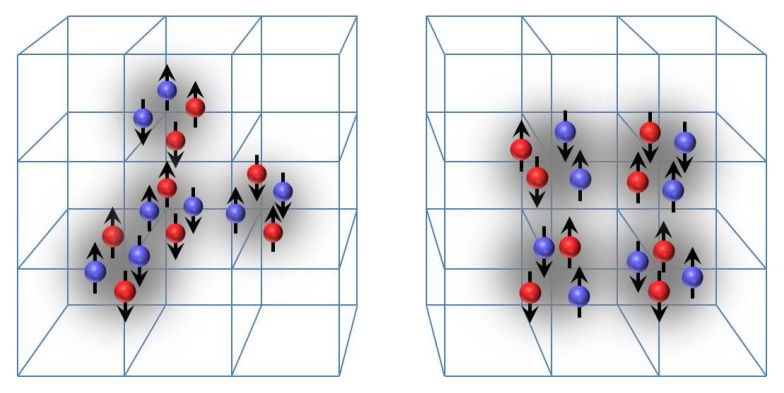
\includegraphics[scale=.7]{Picture13.png}}
    \caption{Схематическое изображение начальных состояний $\alpha$ -кластера с тетраэдрической и планарной конфигурациями}
    \label{fig14}
\end{figure}

Спустя несколько лет Моринага предположил, что несферические и даже линейные цепочки $\alpha$-кластеров могут описывать некоторые состояния $\alpha$-подобных ядер (Morinaga, 1956). Одним из кандидатов на такое описание было второе состояние 0$^{+}$ $^{12}$C, постулированное Хойлом (Hoyle, 1954) как ответственное за усиление тройной $\alpha$-реакции в звездах и экспериментально наблюдаемое вскоре после этого (Cook et al., 1957). Одновременно с этими теоретическими разработками новые эксперименты предоставили высококачественные данные об упругом $\alpha$-$\alpha$-рассеянии (Афзал и др., 1969; Гейденбург и Теммер, 1956; Нильсон и др., 1958). Это, в свою очередь, привело к развитию эффективного $\alpha$-$\alpha$ взаимодействия (Али и Бодмер, 1966). 

Примерно в то же время Бринк использовал детерминантную волновую функцию Марньо Слейтера для $\alpha$-кластера и метод координат генератора, чтобы упростить вычисления, которые были трудными в более общем формализме метода резонирующих групп (Brink, 1966a). Эквивалентность метода координат генератора и метода резонирующих групп была позже выяснена Хориучи (Horiuchi, 1970). Что касается $\alpha$-распадов, Кларк и Ван вычислили вероятность образования $\alpha$-кластеров вблизи поверхности тяжелых ядер (Clark and Wang, 1966). Между тем Икеда, Такигава и Хориучи заметили, что $\alpha$-кластеризация появилась близко к порогам $\alpha$-распада, и они были схематично обозначены так называемыми диаграммами Икеда (Ikeda et al., 1968). Следуя этим же концепциям, изучение кластеризации было расширено на богатые протонами и нейтронно-богатые системы с близкими открытыми порогами. В соответствующих состояниях являются слабо связанными системами кластеров и избыточных нейтронов или протонов. 

Был опубликован ряд обзоров кластеризации ядер (Akaishi et al., 1986; Beck, 2010, 2012, 2014; Freer, 2007; Funaki et al., 2015; Horiuchi et al., 2012; von Oertzen et al. , 2006). Из-за нехватки места невозможно подробно охватить все области исследований. Тем не менее, мы стараемся дать сбалансированный взгляд на поле с точки зрения команды практиков, владеющих целым рядом методов и опытом. В обзоре теоретических методов мы сосредотачиваемся на микроскопической кластеризации, когда кластеры возникают из нуклонных степеней свободы. Поскольку эта область динамична и развивается, некоторые ключевые вопросы в настоящее время не решены, и существуют разногласия между различными методами. Более того, некоторые из наиболее интересных результатов, вероятно, будут получены в ближайшем будущем. Этого следовало ожидать в растущей области, где многие активно занимаются важными открытыми вопросами и исследованиями. Полезно кратко суммировать сильные стороны и проблемы различных теоретических подходов. Большинство обсуждаемых нами методов представляют собой вариационные вычисления с использованием некоторого предписанного анзаца для ядерной волновой функции. Они включают в себя антисимметризованную молекулярную динамику, фермионную молекулярную динамику, в Tohsaki-Хориучи - волновая функция и модель контейнера Шук-Репка, и микроскопические модели кластера, используя резонирующую группу или генератор координат методов. Эти вариационные подходы часто дают хорошее согласие с экспериментальными данными, а также интуитивную картину лежащих в основе ядерных волновых функций. Основные задачи состоят в том, чтобы включить первые принципы ядерных сил и устранить систематические ошибки, связанные с выбором вариационных базисных состояний.

Некоторые вариационные методы также были объединены с методами Монте-Карло. Вариационный Монте-Карло использует стохастическую выборку для вычисления интегралов перекрытия. Он также часто используется в качестве отправной точки для моделирования диффузии или моделирования Монте-Карло с помощью функции Грина. В этих расчетах использовались ядерные силы из первых принципов, и систематические ошибки можно оценить, допустив неограниченную эволюцию квантовой волновой функции. Основная задача для этих расчетов является то, что вычислительные затраты экспоненциально возрастает с увеличением числа частиц. Другой метод, называемый оболочечной моделью Монте-Карло, использует вспомогательное поле Монте-Карло для выбора оптимизированных состояний вариационного базиса. Как и в случае с другими вариационными методами, проблема заключается в систематических ошибках из-за выбора базисных состояний. 

Богатство тюркского языка доказано множеством фактов. Выходящие из народной среды талантливые поэты не должны выявлять свои способности на персидском языке. Если они могут творить на обоих языках, то все же очень желательно, чтобы они на своем языке писали стихов побольше". И далее: "Мне кажется, что я утвердил великую истину перед достойными людьми тюркского народа, и они, познав подлинную силу своей речи и её выражений, прекрасные качества своего языка и его слов, избавились от пренебрежительных нападок на их язык и речь со стороны слагающих стихи по-персидски.

Модель оболочки без ядра с расчетами континуума начинается с первых принципов ядерных сил, описываемых киральной эффективной теорией поля, и продемонстрировала впечатляющее согласие свойств континуума легких ядер. Подобно функции Грина Монте-Карло, проблема этого метода заключается в экспоненциальном масштабировании усилий при работе с более крупными системами. Модель оболочки без ядра, адаптированная к симметрии, предлагает несколько многообещающих идей для эффективной мобилизации вычислительных ресурсов на основе симметрии. Тем не менее остаются трудности в достижении более крупных систем с использованием ядерных сил из первых принципов.

Теория эффективного поля ядерной решетки использует киральную теорию эффективного поля и методы решеточного Монте-Карло для определения ядерной структуры, рассеяния и реакций. Его преимущество заключается в относительно мягком масштабировании с размером системы и общей платформе для обработки систем с несколькими и многими телами при нулевой и ненулевой температуре. Однако есть дополнительная трудность при работе с решеткой с нарушенной вращательной симметрией, и шаг решетки необходимо уменьшить, чтобы уменьшить систематические ошибки.
Мы также упоминаем несколько других недавних исследований. В одной недавней работе состояния $^{12}$C рассматриваются в модели Скирма (Lau and Manton, 2014). Хотя расчеты хорошо согласуются с измеренным экспериментальным спектром, подробная связь с лежащими в основе ядерными силами еще не полностью реализована. В то время как недостатки оболочечной модели в описании кластерных структур были известны с ранних лет, объяснение ядерной кластеризации как возникающего коллективного явления вблизи открытых порогов дается в работе \cite{5}. (Okolowicz et al., 2013), рассматривая ядро как открытую квантовую систему, взаимодействующую через близлежащие состояния континуума.


\section{ Последные экспериментальные результаты}
\hspace{0.6cm}
Экспериментальный материал получен с помощью 1-метровой водородной пузырьковой камеры ЛВЭ ОИЯИ, облученной ядрами кислорода с импульсом 3,25 А ГэВ/с на Дубненском синхрофазотроне и основывается на статистике $\sim$14500 измеренных $^{16}$Op-событий. Идентификация $\pi^{+}$-мезонов и протонов проводилась визуально в области импульсов р<1,2 ГэВ/c. При изучении реакции  рассматривались события, в которых измеренная длина треков двух- и шестизарядных фрагментов превышала 35 см, что было необходимо для их надежной идентификации по массе. При такой длине треков средняя относительная погрешность определения импульсов фрагмента не превышает 3,5\%, а углы вылета измеряются с точностью $\Delta\theta<0,1^{\circ}$. Разделение фрагментов по массе проводилось по величине их импульса: фрагменты с зарядом $z_{f}$=2 в интервале импульса р=(1,8$\div$15,0) ГэВ/с относились к $\alpha$-частице, а c $z_{f}$=6 и р=(36,5 $\div$ 44,0) ГэВ/с  к $^{12}$C. Другие вопросы, связанные с обработкой стереофотографий с 1 метровой водородной пузырьковой камеры, восстановлением пространственных координат, а также с вычислением кинематических характеристик частиц и фрагментов, описаны в работах \cite{1}-\cite{4}.

Экспериментальное изучение роли кластеризации в ядрах восходит к самым ранним наблюдениям $\alpha$-распада тяжелых ядер. В ранних моделях ядер многие предполагали, что $\alpha$-частица может играть важную роль, например, работа Хафстада и Теллера в 1938 г. (Hafstad and Teller, 1938) хорошо описывает возможные структуры ядер, таких как $^{8}$Be , $^{12}$C и $^{16}$O, построенные из $\alpha$-частиц. В этой ранней работе также высказывались предположения о существовании молекулярных структур в легких ядрах, где нейтроны или даже нейтронные дыры могут обмениваться между ядрами $\alpha$-частиц. Эти основные идеи остаются движущими силами для большей части нынешней экспериментальной программы. Катализатором "современной" эры кластеризации ядер послужили идеи Моринаги в 1956 году, который предположил, что состояние Хойла с энергией 7,65 МэВ при $^{12}$C, которое недавно было измерено экспериментально, могло быть линейным расположением 3$\alpha$-частиц (Morinaga, 1956). Идея о том, что линейные цепные структуры могут существовать в ядрах, до сих пор остается актуальной и остается нерешенной. Эксперимент был в значительной степени мотивирован желанием предоставить доказательства типов структур, предусмотренных Моринага и рассчитанных Бринком с использованием модели альфа-кластеров Блоха-Бринка (Brink, 2008; Brink and Boeker, 1967). Например, в случае $^{12}$C модель $\alpha$-кластера обнаруживает две структуры. Первый - это равностороннее треугольное расположение, которое исторически ассоциировалось с основным состоянием, а второе - линейное расположение (или цепочка).

\begin{figure}[!ht]
\includegraphics{Picture10.png}
\caption{Расчетный спектр состояний $^{16}$O в предположении динамической симметрии T$_{d}$d, полученный с использованием алгебраической кластерной модели (Bijker, Iachello, 2014)}
\label{fig10}
\end{figure}

Возможность экспериментов выяснить кластерные структуры легких и тяжелых ядер определяется диапазоном экспериментальных наблюдаемых, которые могут быть извлечены. С упрощенной отправной точки, момент инерции вращающегося ядра дает представление о деформации, которая может быть, по крайней мере, показана как совместимая с кластерной структурой, даже если не является прямым доказательством. Если использовать 8 Be в качестве примера, то вращательная полоса основного состояния имеет состояния 0$^{+}$, 2$^{+}$ и 4$^{+}$ при 0, 3,06 и 11,35 МэВ. Отношение энергии 4$^{+}$ к 2$^{+}$ составляет 3,7, что очень близко к тому, что можно было бы ожидать для вращающегося ядра, 3,33. Момент инерции, извлекаемый из E$_{rot}$=J(J+1)$\sim$2/2I, соизмерим с моментом, найденным в расчетах  методом Монте-Карло, которые четко раскрывают структуру кластера. Мы обсуждаем вычисления с использованием функции Грина Монте-Карло в подразделе VI.B. В качестве простого руководства, значение $\sim$ 2/2I, связанное с состоянием 2$^{+}$, составляет 0,51 МэВ, что даже при простом вычислении дает разделение двух $\alpha$-частиц на удвоенный радиус $\alpha$-частицы. Наблюдение за серией состояний, лежащих во вращательной последовательности, не является водонепроницаемым свидетельством кластеризации или деформации. Здесь измерения сил электромагнитных переходов обеспечивают проверку перекрытия структур в начальном и конечном состоянии и степени коллективности. Для случая $^{8}$Be измерение силы перехода B(E$_{2}$) из состояния 4$^{+}$ в состояние 2$^{+}$ обеспечивает согласованное описание как с вращательной картиной, так и с расчетами.

\begin{figure}[!ht]
\centerline{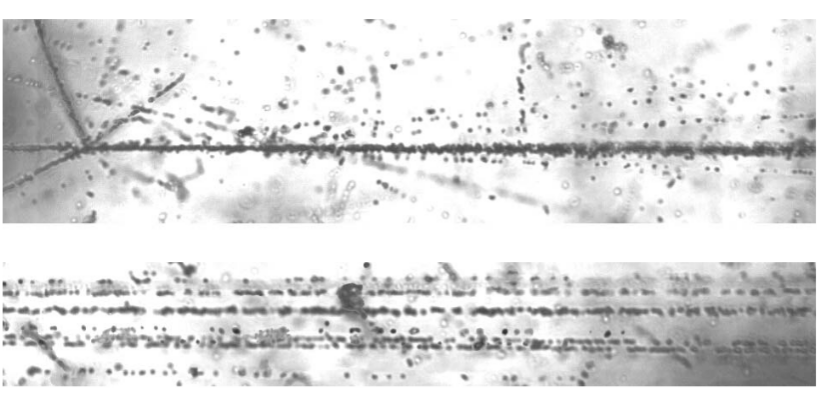
\includegraphics[scale=.6]{Picture1.png}}
\caption{Фрагментации ядра $^{28}$Si c энергией 3,65A ГэВ в ядерной эмульсии.}
\label{fig1}
\end{figure}

Однако, как отмечалось выше, к этой упрощенной интерпретации следует относиться с осторожностью. Во-первых, все состояния в 8-Be не связаны и, следовательно, встроены в континуум и, следовательно, будут иметь вклады континуума. Во-вторых, ширина состояний значительна и, соответственно, время жизни короткое, и поэтому понимание того, что означает коллективность в таких коротких временных масштабах, неясно. Наконец, многие вычисления используют приближения связанных состояний и, следовательно, не могут быть полностью точными. Существует интересное обсуждение значения вращательных полос, в которых резонансы встроены в континуум, с акцентом на 8 Be Гарридо и др. (Гарридо и др., 2013). Вывод состоит в том, что вращательные полосы, встроенные в континуум, все еще могут быть значимой концепцией, но что континуум влияет на такие свойства, как вероятности переходов, и, следовательно, здесь к континууму нужно обращаться осторожно. Это особенно важно для сравнения с методами КФИМ.

Ширина состояния показывает значительное количество деталей, касающихся структуры и распада. Чем больше перекрытие исходной структуры с перегородкой распада, тем короче время жизни и больше ширина. В случае возбуждения 2$^{+}$ $^{8}$Be ширина составляет 1,5 МэВ. На ширину распада также влияет барьер, через который распад должен проходить, но если убрать кулоновский и центробежный барьеры, то уменьшенную ширину можно сравнить с пределом Вигнера. Это значение, которое должна принимать уменьшенная ширина, если $\alpha$-частицы полностью предварительно сформированы. Для этого конкретного состояния было обнаружено, что экспериментальная ширина очень близка к пределу Вигнера, что снова указывает на существование кластерной структуры (Cerny, 1974; Overway et al., 1981). Еще одна сигнатура, недоступная для распада примерных состояний в $^{8}$Be, - это измерение доминирующего канала распада. Состояния с сильными кластероподобными свойствами должны предпочтительно распадаться за счет излучения кластера, а не, например, распада протона или нейтрона. В реакциях это структурное сходство может быть описано с помощью спектроскопического фактора или асимптотического нормировочного коэффициента.

В следующих разделах мы исследуем многие недавние достижения в экспериментальном исследовании кластеризации ядер. Во многих случаях недавние работы основываются на значительных исторических трудах. Существует множество обзорных статей, описывающих развитие предмета, и мы отсылаем читателя к следующим источникам: (Beck, 2010, 2012, 2014; Freer and Fynbo, 2014; Freer and Merchant, 1997; Freer, 2007; von Oertzen et al. др., 2006).

\section{ Состояние исследований легких ядер}
\hspace{0.6cm}
Безусловно, наибольшее экспериментальное внимание было уделено изучению кластерной структуры $\alpha$-сопряженных ядер. Здесь проблема заключалась в том, чтобы сначала обеспечить более глубокое понимание природы кластерных структур и, в конечном итоге, определить, действительно ли цепные состояния существуют в легких ядрах или нет. Конечная цель состоит в том, чтобы определить экспериментальные характеристики, чтобы их можно было проверить с помощью Каскадно-фрагментационная испарительная модель или других микроскопических расчетов.

\begin{figure}[!ht]
\centerline{\includegraphics[scale=.6]{picture8.png}}
\caption{Одномерная корреляционная функция C (q), приведенная в (1) для альфа-частиц, испускаемых в столкновениях $^{16}$O-p при 3,25 A ГэВ/c. Сплошная кривая является результатом минимальной $\chi^{2}$ аппроксимации экспериментального спектра C (q) функцией (2).}
\label{fig12}
\end{figure}

Как уже было описано, одним из лучших примеров сравнения между КФИМ теорией и экспериментом является измерение гамма-распада состояния 4$^{+}$ в $^{8}$Be в состояние 2$^{+}$ (Datar et al., 2013). Это был тур-де-сила, где наблюдалась ветвь гамма-распада $\sim$ 10$^{-7}$. В эксперименте использовалась мишень с газовой струей гелия, а состояние 4$^{+}$ резонансно заселялось пучком $^{4}$He. Испускаемое гамма-излучение и последующее испускание двух $^{+}$-частиц от распада состояния 2$^{+}$ были обнаружены при тройном совпадении. Наблюдалось поперечное сечение 165 (54) нб, что переводилось в B (E$_{2}$) 25 $\pm$ 8 e$^{2}$ фм$^{4}$. Это очень близко к последнему вычисленному в методе GFMC значению 26,0 $\pm$ 0,6 e$^{2}$ фм $^{4}$ (Datar et al., 2013). Эти последние расчеты, как известно, показали, что основное состояние 8-Be сильно кластеризовано, и со значительной точностью предсказали спектр энергии возбуждения (Wiringa et al., 2000). Учитывая, что B (E2) чувствителен как к перекрытию распределения зарядов, так и к коллективному поведению, такой результат можно рассматривать как свидетельство как кластерного, так и коллективного поведения. Однако в этом случае возникает довольно интересная загадка. Ширина состояний 2$^{+}$ и 4$^{+}$ велика (1,5 и 3,5 МэВ соответственно). Из принципа неопределенности это соответствует времени жизни порядка 10$^{-22}$ секунды. Это время пролета нуклона с энергией Ферми через ядро. Как могут развиваться коллективные процессы и возникать ротационное поведение при очевидном несоответствии во временных масштабах и что означает ротация в таких системах (Fossez et al., 2016). Когда дело доходит до точного описания свойств таких состояний, встроенных в континуум, необходимо полностью учитывать влияние континуума на свойства перехода (Garrido et al., 2013), и очень важно, чтобы методы КФИМ были разработаны для такие несвязанные системы.

Состояние Хойла в $^{12}$C - одно из наиболее известных состояний в ядрах, учитывая его довольно важную роль в синтезе углерода посредством тройного $\alpha$-процесса. Недавний обзор этого состояния (Freer and Fynbo, 2014) дает исчерпывающее описание его роли в синтезе и его экспериментальных свойств. Достаточно сказать, что с экспериментальной точки зрения эти свойства хорошо изучены. С другой стороны, его структура менее изучена.

Тот факт, что в расчетах модели оболочки без ядра не удается воспроизвести энергию состояния Хойла (Navr\`{a}til et al., 2007, 2000b), без использования значительно расширенного базиса гармонических осцилляторов, уже указывает на то, что структура лежит за пределами того, что легко описывается модель оболочки. Первый расчет состояния Хойла был проведен всего несколько лет назад в \cite{4}. (Эпельбаум и др., 2011). Эти последние вычисления смогли явно зафиксировать $\alpha$-кластеризацию, которая появляется в этом состоянии. Расчеты AMD, рис. 1, показывают, что состояние Хойла представляет собой расширенную трех $\alpha$-систему и что связанные с ней возбужденные состояния 2$^{+}$ и 4$^{+}$ не являются жесткими, вращательными, возбуждениями и что рыхлая совокупность $\alpha$-частиц, -газ, может быть лучшее описание. К аналогичному выводу пришли расчеты фермионной молекулярной динамики (ФМД\nomenclature{ФМД}{фермионная молекулярная динамика}) для тех же состояний (Neff, Feldmeier, 2014). Здесь было высказано предположение, что резонансы 2$^{+}$ и 4$^{+}$ могут рассматриваться как члены вращательной полосы, построенной на основном состоянии $^{8}$Be, где третья $\alpha$-частица вращается вокруг ядра $^{8}$Be с относительным орбитальным угловым моментом 2 или 4 соответственно. Происхождение ядерных кластеров, имеющих отношение к образованию состояния Хойла, также обсуждается Okolowicz et al. (Okolowicz et al., 2013).

Баркер и Трейси (Barker and Treacy, 1962) заметили, что для воспроизведения ширины состояния Хойла необходимо использовать необычно большой радиус: с радиусом 1,6 фм A 1/3, шириной 9,3 эВ соответствует безразмерной приведенной ширине $\theta_{2}$ = $\gamma\lambda 2 M_{red}R_{2}/2\sim 2$ , равной 1,5. Следовательно, ширина состояния Хойла очень велика; это можно понять только при наличии большой степени $\alpha$-кластеризации. Наличие такой кластерной структуры увеличивает сечение $\alpha$-захвата. Но его наличие в окне Гамова приводит к увеличению общего сечения захвата в 10$^{8}$ раз. Без точного местоположения этого состояния количество углерода-12 было бы значительно уменьшено, и, таким образом, оно тесно связано с существованием органической жизни. Довольно глубокий вопрос заключается в том, является ли это счастливой случайностью, или есть какая-то причина, по которой состояния с сильно развитой кластерной структурой должны существовать вблизи соответствующих пороговых значений распада (Epelbaum et al., 2013b, a; Freer and Fynbo, 2014; Okolowicz et al., 2013).

Помимо того факта, что состояние Хойла имеет 3$\alpha$-кластерную структуру, природа этой структуры еще предстоит выяснить. Расчеты AMD на рисунке 1 показывают преобладание $^{8}$Be + $\alpha$ конфигураций в рыхлой сборке, так что 2$^{+}$ и 4$^{+}$ возбуждения не обладают четким вращательным поведением. Расчеты фермионной молекулярной динамики (ФМД) состояния Хойла приводят к аналогичным выводам (Chernykh et al., 2007). Расширением этих идей является то, что состояние может быть описано газом / конденсатом $\alpha$-частиц (Funaki et al., 2009). В принципе, можно получить представление о структуре через свойства распада состояния. В этом случае открыты две моды распада; последовательный и прямой. В последнем случае система не распадается через основное состояние 8-Be. Верхний предел непоследовательного $\alpha$-распада в 4\% был впервые определен в 1994 г. (Freer et al., 1994). Впоследствии измерение реакции $^{40}$Ca + $^{12}$C при 25 МэВ / нуклон показало, что степень разветвления на самом деле была выше и составляла 7,5 $\pm$ 4\%. Это было оспорено дальнейшими измерениями, в которых были предложены верхние пределы всего 5 $\cdot$ 10 $^{-3}$ (95\% CL) (Kirsebom et al., 2012; Manfredi et al., 2012) и 9 (2)$\cdot$ 10$^{-3}$ (Рана и др., 2013). Он был улучшен до 0,2\% (Itoh et al., 2014). Эти измерения теперь достигли чувствительности, при которой эффекты фазового пространства перестают быть доминирующим фактором, и можно исследовать структуру с пределами 0,047\% (Smith et al., 2017) и 0,043\% (Dell'Aquila et al., 2017) по сравнению с прогнозируемым пределом фазового пространства 0,06\% (Smith et al., 2017).

Второй подход заключается в исследовании распределения заряда посредством неупругого рассеяния электронов (Хорикава и др., 1971; Накада и др., 1971; Sick and Mccarthy, 1970; Strehl and Schucan, 1968). В таких измерениях определяется переходный форм-фактор, который исследует перекрытие основного состояния с состоянием Хойла. Для интерпретации таких измерений требуется модель, которая может описывать как основное, так и возбужденное состояния. И описание конденсата (Funaki et al., 2006a), и описание ФМД (Chernykh et al., 2007) указывают на то, что состояние Хойла связано с радиусом, большим, чем у основного состояния, в 1,35-1,60 раза (в зависимости от модель, использованная для анализа данных), что соответствует увеличению объема в 2,5-4 раза. На рисунке 2 показано рассчитанное распределение неупругого рассеяния электронов для модели конденсата (Funaki et al., 2006a).

Третий подход к выводу структуры состояния Хойла - поиск коллективных возбуж-дений, в частности возбуждения 2$^{+}$. Измерения неупругого рассеяния (Freer et al., 2009; Itoh et al., 2011; Zimmerman et al., 2011) были первыми, кто подтвердил наличие такого возбуждения. Общий анализ данных о рассеянии протонов и $\alpha$-частиц в пользу 2$^{+}$-резонанса дан в [5]. (Freer et al., 2012a), и обсуждение влияния этих измерений дано в работе. (Финбо и Фрир, 2011). Форма линии 2$^{+}$, которая была обнаружена в измерениях неупругого рассеяния 12-C ($\alpha$, $\alpha_{0}$) и 12-C (p, p$_{0}$) (Freer et al., 2012a), определила свойства как E$_{x}$ = 9,75 ( 0,15) МэВ при ширине 750 (150) кэВ. Существование 2$^{+}$ -резонанса было подтверждено измерением реакции $^{12}$C ($\gamma$, 3$\alpha$) на установке HI$\gamma$S (Zimmerman et al., 2013). Функция возбуждения для этих измерений показана на рисунке 3 и дает резонансные параметры E$_{x}$= 10,13 (6) МэВ и $\Gamma$ = 2,1 (3) МэВ (Zimmerman, 2013).

\begin{figure}[!ht]
\centerline{\includegraphics[scale=.5]{picture3.png}}
\caption{Рассчитанный неупругий форм-фактор для неупругого рассеяния электронов из основного состояния 0$^{+1}$ в возбужденное состояние 0$^{+2}$ (Funaki et al., 2006a) для подхода Конденсата Бозе — Эйнштейна (красный) по сравнению с экспериментальным данные из исх. (Horikawa et al., 1971; Nakada et al., 1971; Sick and Mccarthy, 1970; Strehl and Schucan, 1968).}
\label{fig1}
\end{figure}


\begin{figure}[!ht]
\centerline{\includegraphics[scale=.5]{picture4.png}}
\caption{(а) Измеренные сечения E$_{1}$ и E$_{2}$ реакции $^{12}$C ($\gamma$, $\alpha_{0}$) $^{8}$Be. (b) Измеренный относительный фазовый угол E$_{1}$-E$_{2}$ ($\varphi$ 12) вместе с фазовым углом, рассчитанный по двухрезонансной модели (Zimmerman et al., 2013).}
\label{fig3}
\end{figure}
Эти измерения теперь расширены до более высоких энергий и продолжают ожидаемую тенденцию для возбуждения 2$^{+}$. Если состояние имеет вращательное поведение, тогда также должно быть состояние 4+, близкое к 14 МэВ. Существуют предварительные доказательства такого состояния при 13,3 МэВ и ширине 1,7 МэВ (Freer et al., 2011; Jyv$\ddot{a}$skyl$\ddot{a}$, 2013; Ogloblin et al., 2014). Существование этого последнего состояния еще предстоит окончательно подтвердить. Похоже, что он сильно распадается на основное состояние 8-Be, в отличие от возбужденного состояния 2$^{+}$, что может дать представление о том, как строится угловой момент, то есть через вращение $\alpha$-частицы вокруг 8-Be (0$^{+}$) ядро. Хотя был достигнут большой прогресс в понимании структуры 12-C, измерения обычно являются сложными и часто далеко не однозначными. Таким образом, потребность в подробной спектроскопии сохраняется. Здесь подход Орхусской группы (Kirsebom et al., 2014) к измерению электромагнитных свойств указывает путь для этих будущих исследований. Реакция захвата p + $^{11}$B используется для резонансного заселения состояний при $^{12}$C, и их распад после испускания ненаблюдаемого гамма-распада регистрируется через следующий канал заряженных частиц.

Состояние Хойла, хотя и расширенное, не согласуется с линейной структурой цепочки, которая требует, чтобы состояние 2$^{+}$ лежало на $\sim$1 МэВ ниже, чем наблюдаемое экспериментально. Теоретические указания (Kanada-En'yo, 2007) предполагают, что состояние 10,3 МэВ, 0$^{+3}$является наилучшей возможностью. Это состояние имеет ширину 3 МэВ, и можно ожидать, что состояние 2$^{+}$, соответствующее линейной цепочечной структуре, близко к 11,5 МэВ, и будет иметь очень большую ширину. Пока такое состояние еще предстоит наблюдать. Недавно Ито и др. Экспериментально сообщили о возможности двух состояний 0+ около 10 МэВ. (Itoh et al., 2011) и поддерживается расширенным расчетом Tohsaki-Horiuchi-Schuck-R$\ddot{o}$pke (THSR) (Funaki, 2015; Funaki et al., 2015).

На рис.\ref{fig3} показана компиляция теоретических спектров и переходов для состояний 0$^{+}$ и 2$^{+}$ в сравнении с экспериментальными данными. Хотя существует множество не- и полумикроскопических расчетов 3$\alpha$, мы показываем только микроскопические расчеты с полностью антисимметризованными волновыми функциями и нуклон-нуклонными взаимодействиями. Трудно напрямую сравнивать качество воспроизведения микроскопических расчетов с немикроскопическими расчетами, где взаимодействия (или гамильтониан) обычно феноменологически корректируются, чтобы соответствовать энергетическим спектрам 12-C. Следует также отметить, что мы не должны обсуждать  вычисления. полученные из реальных ядерных сил на одной основе с расчетами с использованием феноменологических эффективных ядерных взаимодействий.  В 3$\alpha$RGM (Kamimura, 1981), расширенном КФИМ(Funaki, 2015; Funaki et al., 2015), 3$\alpha$GCM (Descouvemont, Baye, 1987; Suhara, Kanada-En'yo, 2015; Uegaki et al., 1979), и 3$\alpha$+ p 3/2 (Suhara, Kanada-En'yo, 2015) используются феноменологические эффективные ядерные взаимодействия волковских сил (Волков, 1965). Параметры взаимодействия сил Волкова настроены так, чтобы воспроизвести $\alpha$-$\alpha$-рассеяние, хотя между этими расчетами есть небольшие различия в параметрах. Результаты AMD (Kanada-En'yo, 1998a, 2007) получены с использованием силы MV1 (Ando et al., 1980), которая представляет собой феноменологическое эффективное ядерное взаимодействие, модифицированное на основе силы Волкова для описания свойств насыщения, тогда как Результаты ФМД + 3$\alpha$ (Черных и др., 2007) получены на основе реалистичного аргоннского потенциала V18 с феноменологической настройкой. Для расчетов КФИМ (Navratil et al., 2007) и теории эффективного поля ядерной решетки (Epelbaum et al., 2012) показаны результаты, полученные с реалистичными силами NN и NNN, полученными из киральной эффективной теории. В расчетах симплектической модели без ядра (Dreyfuss et al., 2013) используется упрощенный эффективный гамильтониан.

В целом расчеты 3$\alpha$ хорошо описывают энергетические спектры состояний кластера выше порога 3$\alpha$ и формфакторы рассеяния электронов для состояния 0${+1}$ и перехода 0$^{+2}$ $\rightarrow$ 0$^{+1}$, но их недостаточно для описания некоторых свойств низколежащие состояния, такие как расстояние между уровнями 0$^{+1}$ -2$^{+1}$, сила перехода $E_{2}$ для 2$^{+1}$ $\rightarrow$ 0${+1}$ и 0$^{+2}$ $\rightarrow$ 2 1. Гибридные расчеты моделей 3$\alpha$ + p 3/2 и FMD + 3$\alpha$, а также AMD могут разумно описать свойства основной полосы и возбужденные спектры для состояний кластера. 
Лирические стихи трудно поддаются датировке, поскольку отклики на известные нам факты жизни поэта в них улавливаются довольно редко, а событийность для них вообще не свойственна. "Сокровищница мыслей" - лирическая исповедь поэта, передающая всю гамму его переживаний. Наряду с внешним любовным планом в них присутствует высший - по-суфийски спиритуализированный и использующий традиционные образы чувственной лирики в метафорическом ключе. При этом оригинальные метафоры Навои переплетаются с традиционными, почерпнутыми им из богатой традиции восточной поэзии. 
Расчет NCSM не может описать возбужденные состояния кластера выше порога, поскольку эти состояния находятся за пределами модельного пространства, тогда как NCSpM, который содержит более высокие конфигурации оболочки для возбуждений кластера, и вычисления NLEFT описывают структуры кластера в возбужденных состояниях выше порога. например, расстояние между уровнями 0$^{+1}$ - 2$^{+1}$, сила перехода E$_{1}$ для 2$^{+1}$ $\rightarrow$ 0$^{+1}$ и 0$^{+2}$ $\rightarrow$ 2$^{+1}$. Гибридные расчеты моделей 3$\alpha$ + p 3/2 и FMD + 3$\alpha$, а также AMD могут разумно описать свойства основной полосы и возбужденные спектры для состояний кластера. Расчет NCSM не может описать возбужденные состояния кластера выше порога, поскольку эти состояния находятся за пределами модельного пространства, тогда как NCSpM, который содержит более высокие конфигурации оболочки для возбуждений кластера, и расчеты NLEFT описывают кластерные структуры в возбужденных состояниях выше порога. Расчеты ab initio (NCSpM и NLEFT) имеют тенденцию сильно недооценивать размер основного состояния, а также дают малые значения размера и матричного элемента E0 для состояния Хойла. Ширины $\alpha$-распада рассчитаны в 3$\alpha$RGM (Kamimura, 1981) и 3$\alpha$GCM (D) в [5]. (Descouvemont and Baye, 1987) путем решения $^{8}$Be + $\alpha$-рассеяния и оценены в расширенном THSR (Funaki, 2015; Funaki et al., 2015), 3$\alpha$GCM (U) в Ref. (Uegaki et al., 1979) и AMD (Kanada-En'yo, 2007) в рамках приближений связанных состояний с использованием уменьшенных амплитуд ширины. Имеющиеся данные для ширин $\alpha$-распадов количественно или качественно воспроизводятся теоретическими расчетами. Хотя в понимании структуры 12-C был достигнут значительный прогресс, очевидно, что существуют как необходимость, так и возможности для измерений, чтобы более точно ограничить свойства состояний, представленных на рисунке 1. В частности, это требует измерения скорости электромагнитных переходов там, где это возможно.

\addcontentsline{toc}{section}{Выводы к 1 Главе}
\section*{Выводы к 1 Главе}
\hspace{0.6cm}
В заключение приведем основные выводы из анализа сложившейся
экспериментальной и теоретической ситуации в области фрагментации
релятивистских ядер.
\begin{enumerate}
    \item На основе анализа экспериментальных данных по фрагментации и теории КХД\nomenclature{КХД}{Квантовая хромодинамика} аргументированно доказана общность процессов множественной генерации частиц и фрагментации ядер.
    \item При энергиях 2-3 ГэВ на нуклон наступает режим предельной фрагментации ядер ("ядерный скейлинг"), заключающийся в независимости характеристик процесса от типа налетающей частицы ($\gamma$-квант, нуклон, пион или ядро).
    \item Обнаружены и исследованы процессы кластерного распада легких и промежуточных ядер, указывающие на их динамическую структуру.
    \item Появился ряд модельных подходов, систематизирующих новые явления по фрагментации и кластеризации ядер.
    \item В $^{16}$Ор-взаимодействиях при 3,25 А ГэВ/с исследованы особенности процессов кластеризации с участием легких (А=3) зеркальных ядер и установлена близость кинематических условий их формирования.
\end{enumerate}

\chapter{Методика эксперимента}
\section{Основные характеристики первичного пучка и 1-м ВПК}
\hspace{0.6cm}
Однометровая водородная пузырьковая камера [54; С.1-10. С.1-8.]
(ВПК) облучалась на синхрофазотроне ЛВЭ ОИЯИ пучком ядер кислорода
при импульсе 3,25 А ГэВ/с. Во время облучения камера находилась в
магнитном поле со средней напряженностью H $\approx$ 18,5 кГаусс. Направление магнитного поля обычно выбирается так, чтобы оно было ортогонально направлению первичного пучка. Практически это требование выполняется приблизительно и к тому же в силу различных причин напряженность магнитного поля несколько меняется в течение времени экспозиции. В связи с этим перед каждым облучением (заливки водорода в ВПК), проводилось измерение значений трех компонентов напряженности H$_{x}$ , H$_{y}$ , H$_{z}$. Данные аппроксимировались полиномом Лежандра 7-го порядка и использовались при геометрической реконструкции и кинематическом анализе треков вторичных частиц и фрагментов. Плотность рабочей жидкости (водорода) составляла $\rho$ =(0,0584$\pm$ 0,0001) г/см$^{3}$.

Первичный пучок релятивистских ионов, полученный на синхрофазотроне ЛВЭ ОИЯИ при импульсе 3,25 ГэВ/с на нуклон (3,25 А ГэВ/с), представляет собой смесь ядер $^{16}$О(85\%) и $^{12}$С, $^{14}$N(15\%) [100; С.192-196.]. Кроме того, в рабочую зону камеры могут попасть изотопы азота или кислорода, образовавшиеся при взаимодействии первичного пучка с веществом стенки канала вывода или ограждения ВПК. Такие частицы при визуальном отборе могут быть спутаны с пучковой частицей из-за близости
ионизации и линейной плотности $\delta$-электронов на треке. Поскольку ионизация пропорциональна квадрату заряда иона Z, то уже в ходе просмотра пленок можно разделить треки $^{16}$О и $^{14}$N, отношение плотностей зерен на пленках для которых различается в 1,3 раза (64/49). 

Рабочий объем ВПК  фотографировался посредством четырех фотокамер, оптические оси которых  параллельны друг к другу  и  ортогональны границе   раздела   сред стекло-водород. Базисы фотографирования составляют 500 мм по поперечному и 310 мм по продольному направлению по отношению к ВПК. Фотографируемый объем ВПК равнялся 960х360х295 мм$^{3}$.


Экспериментальный материал был получен с помощью 1-метровой водородной пузырьковой камеры ЛВЭ ОИЯИ, облученной ядрами кислорода с импульсом 3,25 А ГэВ/с на Дубненском синхрофазотроне и основывается на статистике $\sim$14500 измеренных $^{16}$Op-событий. Идентификация $\pi^{+}$-мезонов и протонов проводилась визуально в области импульсов р<1,2 ГэВ/c. При изучении реакции (1)  рассматривались события, в которых измеренная длина треков двух- и шестизарядных фрагментов превышала 35 см, что было необходимо для  надежной идентификации по их массе. При такой длине треков средняя относительная погрешность определения импульсов фрагмента не должна превышат 3,5\%, а углы вылета будут измерятся с точностью $\Delta\theta<0.1^{\circ}$. Разделение фрагментов по их массе проводилось по величине  импульса: фрагменты с зарядом $z_{f}$=2 в интервале импульса р=(10,8$\div$15,0) ГэВ/с относиться к $\alpha$-частице, а c $z_{f}$=6 и р=(36,5 $\div$ 44,0) ГэВ/с  к $^{12}$C. Другие вопросы, связанные с обработкой стереофотографий с 1 метровой водородной пузырьковой камеры, восстановлением пространственных координат, а также с вычислением кинематических характеристик частиц и фрагментов, описаны в работах \cite{4}-\cite{7}.

 Тем самым достигается режим предельной фрагментации ядер, что также означает неизменность изотопического состава фрагментов при возрастании энергии столкновения. Особую ценность для кластерной физики имеют события периферической диссоциации налетающего ядра с сохранением числа нуклонов в области его фрагментации. При энергии налетающих ядер свыше 1A ГэВ вероятность такой диссоциации достигает нескольких процентов. Определение взаимодействий как периферических упрощается благодаря возрастающей коллимации фрагментов. 

Пороги детектирования релятивистских фрагментов отсутствуют, а теряемая ими энергия в детекторах минимальна. Все эти обстоятельства принципиально важны для экспериментальных исследований.

В настоящее время экспериментальные генерации частиц и исследования фрагментации процессов релятивистских множественной ядер являются чрезвычайно важными для решения фундаментальных вопросов физики высоких энергий и релятивистской ядерной физики. Одним из важнейших источников информации о структуре ядер и ее влиянии на состав конечных продуктов реакций, а также роли зарядовообменных процессов при фрагментации ядер является исследование соударений релятивистских ядер с нуклонами и ядрами в полуинклюзивных и максимально приближенных к эксклюзивным реакциях (в условиях 4$\pi$-геометрии, с полной идентификацией фрагментов и измерением их импульсов и углов вылета). Таким требованиям к экспериментальным данным наиболее полно соответствуют эксперименты, выполняемые с помощью пузырьковых камер, экспонируемых в сильных магнитных полях в пучках релятивистских ядер.

В таблице приведено сечение канала (26) в зависимости от числа однозарядных частиц n$_{ch1}$. Видно, что в данном топологическом канале эти фрагменты преимущественно сопровождаются выходом только одной положительной частицы, причем доля протонов (с Р<1,2 ГэВ/с) среди них составляет $\sim$80\%. 


\begin{table}
\centering
    \begin{tabular}{|c|c|c|c|}
    \hline
        n$_{ch1}$&	1&	3&	5\\
        \hline
s, в мбн.&	8,94$\pm$0,62&	1,12$\pm$0,20&	0,09$\pm$0,06\\
\hline
    \end{tabular}
    \caption{Сечение канала (26) в зависимости от числа однозарядных частиц n$_{ch1}$}
    \label{tab:my_label}
\end{table}

\hspace{0.6cm}Представленные в настоящей диссертационной работе физические результаты основываются на анализе экспериментальных данных по кислород-протонным взаимодействиям при 3,25 ГэВ/с на нуклон, которые были получены с помощью 1 м водородной пузырьковой камеры (ВПК\nomenclature{ВПК}{Водородная пузырьковая камера}) в
рамках сотрудничества с Лабораторией высоких энергий (ЛВЭ)
Объединенного института ядерных исследований (ОИЯИ). ВПК ЛВЭ ОИЯИ
экспонировалась в пучке релятивистских ядер кислорода на Дубненском
синхрофазотроне.

Методика пузырьковых камер при изучении множественной генерации
частиц и процессов фрагментации ядер в адрон- и ядро-ядерных соударениях при высоких энергиях имеет ряд достоинств, а именно, возможность разделения частиц и фрагментов (ядра-снаряда) по зарядам, что невозможно в экспериментах с фотоэмульсиями без магнитного поля, с хорошей точностью определения их импульса в условиях близких к 4$\pi$-геометрии.

Основными недостатками пузырьковых камер являются, во-первых, их
низкое быстродействие и длительный процесс обработки стереоснимков; во-вторых, невозможность регистрации медленных фрагментов ядра-мишени
из-за малости длины их пробега в рабочем объеме камеры (L $\le$0,2-0,3 см.).

Известными достоинствами ВПК является высокая точность импульсных и угловых измерений, наблюдаемость акта взаимодействия, хорошее пространственное разрешение, соответствующее 4$\pi$-геометрии, надежная идентификация фрагментов по ионизации и импульсам, а также, в силу уникальности эксперимента с налетающим ядром, возможность
регистрации мало энергичных в системе покоя ядра кислорода заряженных
частиц, включая испарительные. Эксперименты в водородной камере дают
дополнительное преимущество поскольку, в отличие от других
экспериментов, рабочая жидкость (мишень) является однородной по
химическому составу и не вносит неопределенностей, связанных, как, например, в фотоэмульсии со статистическим разделением вкладов ядер-мишеней на компоненты с определенным массовым числом. \nomenclature{А ГэВ/с}{Единица измерения импульса релятивистских ядер, приходящегося на один нуклон ядра}


\section{Диссоциация релятивистских ядер}
\hspace{0.6cm}

Импульсное и угловое распределения протонов в событиях топологического канала (26) без каких-либо ограничений на длину треков многозарядных фрагментов приведены на рис.8 и 9. Как видно из рис.1, что импульсное распределение протонов имеет максимум при малых значениях импульса (р$_{p}\sim$225 МэВ/с), и далее наблюдается его быстрый спад до рр<500 МэВ/с, а, начиная с рр>500 МэВ/с темп спада существенно замедляется, продолжаясь вплоть до максимального значения импульса идентификации протонов (р$_{p}$<1200 МэВ/с).

\begin{figure}[!ht]
\centering
\includegraphics[scale=.8]{Picture151.png}
\caption{ Импульсное распределение протонов.}
\label{figon}
\end{figure}

\begin{figure}[!ht]
\centering
\includegraphics[scale=.8]{Picture152.png}
\caption{ Угловое распределение протонов.}
\label{figdeu}
\end{figure}



Эмульсионная камера собирается как стопка слоев с толщиной около 550 мкм и размерами 10х20 см$^{2}$ (рис. 4). Факторами получения значительной статистики событий оказываются толщина, которая достигает 80 г/см$^{2}$ вдоль длинной стороны, и полная эффективность детектирования заряженных частиц. В ядерной эмульсии содержатся в близких концентрациях как тяжелые ядра Ag и Br, так и ядра H. По плотности водорода ядерная эмульсия близка к жидководородной мишени. Эта особенность позволяет сравнивать в одинаковых условиях развалы ядер-снарядов как в результате дифракционной или электромагнитной диссоциации на тяжелом ядре-мишени, так и в результате столкновений с протонами. 


\begin{figure}[!ht]
\centerline{\includegraphics{picture5.png}}
\caption{Инвариантные сечения  дейтронов ($\bullet$) вылетающих в заднюю полусферу ($v_{lab}>90^{\circ}$) в зависимости от их кинетической энергии в системе покоя ядра кислорода в $^{16}$Ор-взаимодействиях при импульсе 3,25 ГэВ/с на нуклон. Сплошная кривая – результат аппроксимации экспериментальных данных в кумулятивной области  МэВ функцией $b(P) = A_{0}\exp^{-B_{0}P^{2}}$.}
\label{fig4}
\end{figure}

Фрагменты релятивистского ядра сосредоточены в конусе, ограниченном углом
\begin{equation}
    \sin\theta_{fr}=\frac{p_{fr}}{p_{0}}
    \label{1}
\end{equation}
где $p_{fr}$ = 0,2 ГэВ/c – величина, характеризующая Ферми-импульс нуклонов, а $p_{0}$ – импульс на нуклон ядра-снаряда. Если пучок направляется параллельно плоскости слоев, следы всех релятивистских фрагментов остаются достаточно долго в одном слое для 3-мерной реконструкции. Распределение событий по каналам взаимодействий с различным составом заряженных фрагментов (или зарядовая топология) является центральной характеристикой фрагментации релятивистских ядер. Результаты по зарядовой топологии когерентной диссоциации для релятивистских ядер 16-O, 22-Ne, 24-Mg, 28-Si и 32-S суммированы в работе [46].

В ядерной эмульсии угловое разрешение для следов релятивистских фрагментов составляет величину порядка 10$^{-5}$ рад. Измерения полярных углов вылета фрагментов $\theta$ оказываются недостаточными для сравнения данных при различных значениях начальной энергии ядер. Более универсальным является сравнение по величинам поперечных импульсов $P_{T}$ фрагментов с массовым числом $A_{fr}$ согласно приближению
\begin{equation}
    P_{T}=A_{fr}p_{0}\sin\theta
    \label{2}
\end{equation}
что соответствует сохранению фрагментами скорости первичного ядра (или импульса на нуклон P$_{0}$ ). Очевидно, что наибольшее значение имеет разрешение по углу $\theta$, распределение по которому "прижато" к нулю. Для ядер с $\alpha$-кластерной основой является оправданным предположение о соответствии релятивистского фрагмента с зарядом $Z_{fr}$= 2 изотопам $^{4}$He.


\begin{figure}[!ht]
\centerline{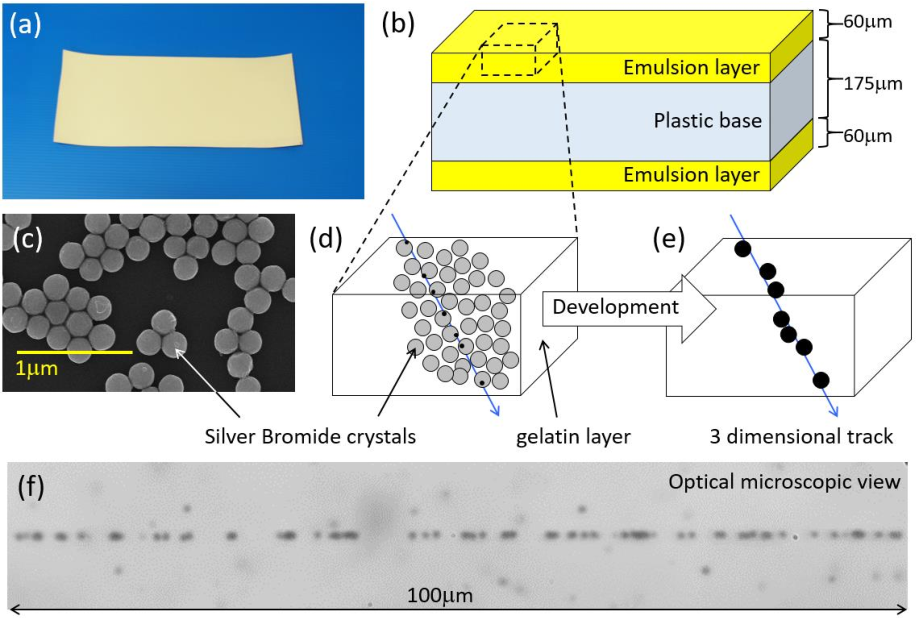
\includegraphics[scale=.4]{Figure1-1.png}}
\label{figure1-1}
\caption{(a) Изображение ядерной эмульсии; (b) Иллюстрация структуры ядерной эмульсии; (c) изображение, полученное с помощью электронного микроскопа, кристаллов бромида серебра в ядерной эмульсии, полученной в университете Нагоя. Диаметр кристаллов составляет приблизительно 200 нм; (d) и (e) Принцип обнаружения заряженной частицы проходит через ядерную эмульсию. Черные маленькие кристаллы бромида серебра в виде точек на рисунке (d) показывают сигнал, прошедший через частицы; (е) Изображение трека, состоящего из частиц серебра, с помощью аноптического микроскопа.}
\end{figure}

Для нейтронодефицитных ядер требуется разделение изотопов 3-He и 4-He. При фрагментации ядер состава эмульсии могут наблюдаться сильноионизирующие фрагменты мишени (рис. 2), включая $\alpha$-частицы, протоны с энергией ниже 26 МэВ и легкие ядра отдачи – n$_{b}$ (b-частицы), а также нерелятивистские протоны с энергией свыше 26 МэВ – n$_{g}$ (g-частицы). Кроме того, реакции характеризуются множественностью мезонов, рожденных вне конуса фрагментации – n$_{s}$ (s-частицы). По этим параметрам можно сделать вывод о характере взаимодействия. В событиях когерентной диссоциации отсутствуют как фрагменты ядер мишени (n$_{b}$ = 0, n$_{g}$ = 0), так и заряженные мезоны (n$_{s}$ = 0). События такого типа из-за отсутствия следов сильноионизирующих частиц nh (nh = nb + ng ) получили неформальное наименование "белых" звезд. "Белые" звезды возникают при ядерном дифракционном и электромагнитном взаимодействии на тяжелых ядрах мишени. Их доля от общего числа неупругих событий составляет несколько процентов. Название "белые" звезды удачно отражает также "срыв" ионизации при переходе от следа первичного ядра к узкому конусу вторичных следов вплоть до Z$_{pr}$ раз. Эта особенность составляет основную трудность для электронных методов, поскольку чем больше в событии степень диссоциации, тем труднее его зарегистрировать. В ядерной эмульсии ситуация совершенно обратная. 	
\section{Сечения $^{16}$Ор-взаимодействий}
\hspace{0.6cm}

В результате просмотра в рабочей зоне камеры, составляющей 44 см,
найдено 14400 $^{16}$Ор-взаимодействий на 39847 пучковых частиц. Когда плотности жидкого водорода $\rho$=0.0584 $\pm$0.0001 г/см$^{3}$, полное наблюдаемое сечение составило $\sigma_{tot}$=375 $\pm$ 9 мбн. Оно требует уточнения и поправок из-за незарегистрированных событий. В первую очередь–это упругие события,
характеризующиеся малыми углами отклонения вторичного трека. Для
оценки числа потерянных двухлучевых событий было проанализировано
распределение по переданному протону-мишени 4-импульсу. Экстраполируя
распределение $d\sigma/dt$ в область $|t|$=0 и учитывая, что доля упругих рассеяний составляет $\sim$1/2 общего числа двухлучевых событий, можно получить нижнее значение сечения потерь – 20 $\pm$2 мбн [106; С.648-655.] и, соответственно, полное сечение $^{16}$Ор-взаимодействий $\sigma_{tot}$=395$\pm$10 мбн. Когда
учтены всех поправок и корректировок на потери событий при просмотре, неизмеримостью коротких, летящих в бок протонов отдачи и доли упругих
рассеяний среди двухлучевых событий неупругое сечение $^{16}$Ор-
взаимодействий оказалось равным $\sigma_{in}$=334 $\pm$6 мбн [32; С.2-9.]. Интересно сравнить полученное значение с мировыми данными, в частности, с популярной аппроксимацией мировых данных по неупругим сечениям адрон-ядерных взаимодействий [37; С.85-88.]:
\begin{equation}
    \sigma_{in}(A,T) = 47,29 A^{1/3}(A^{1/3} + 0,039 X - 0,0009X^{2})
\end{equation}
где $X=\sigma_{0}(T)-33$ - параметр разложения $\sigma_{in}(A,T)$ в ряд по степеням Х; А–массовое число ядра-мишени, Т–энергия налетающей частицы, $\sigma_{0}$ (Т)–близкая к полному сечению нуклон-нуклонного или пион-нуклонного взаимодействия, подлежащая определению из близких по энергии первичной частицы экспериментов. В соответствии с [44; С.427-435.] мы взяли $\sigma_{0}$(Т)=42.22 и получили неупругое сечение $^{16}$Ор-взаимодейс-твий равным $\sigma_{in}$ =332$\pm$ мбн, прекрасно согласующееся с нашими данными.

\begin{figure}[!ht]
\centerline{\includegraphics[scale=.95]{picture6.png}}
\caption{Импульсное распределение $dN_{d}/dP$ дейтронов ($\bullet$) вылетающих в заднюю полусферу ($v_{lab}>90^{\circ}$) в системе покоя ядра кислорода в $^{16}$Ор-взаимодействиях при импульсе 3,25 ГэВ/с на нуклон. Сплошная кривая – результат аппроксимации импульсного распределения кумулятивных дейтронов с  МэВ/с в 500 < P < 640 МэВ/с необласти P > 3,89 МэВ/с, содержащей нерегулярность, функцией $b(P) = A_{0}\exp^{-B_{0}P^{2}}$ }
\label{fig26}
\end{figure}

\chapter{Образование многонуклонных систем и ядер }
\section{Исследование процессов фрагментации }
\hspace{0.6cm}
Импульсное и угловое распределения протонов в событиях топологического канала (26) без каких-либо ограничений на длину треков многозарядных фрагментов приведены на рис.8 и 9. Как видно из рис.8, что импульсное распределение протонов имеет максимум при малых значениях импульса (р$_{p}\sim$225 МэВ/с), и далее наблюдается его быстрый спад до р$_{p}$<500 МэВ/с, а, начиная с р$_{p}$>500 МэВ/с темп спада существенно замедляется, продолжаясь вплоть до максимального значения импульса идентификации протонов (р$_{p}$<1200 МэВ/с).

Из рис.9 видно, что спектр протонов по углу вылета в пределах статистических погрешностей остается постоянным в интервале 5$^{0}$<$\theta$<70$^{0}$ , далее наблюдается его быстрый рост с острым максимумом в интервале угла 80$^{\circ}$<$\theta$<85$^{\circ}$. 

Анализ импульсных спектров двух- и шестизарядных фрагментов в топологическом канале (26) показал, что в событиях с n$_{ch1}$=1 и выходом протона (сечение которых составляет 6,82$\pm$0,51 мбн.) в основном, образуются ядра $^{4}$He и $^{12}$C, т.е. в них сохраняются все нуклоны исходного ядра  кислорода. Импульсное и угловое распределения протонов, образованных в этих событиях также имеют максимумы при р$_{p}\sim$225 МэВ/с, и угле выхода $\sim$82$^{\circ}$ в л.с.к.. Все эти экспериментальные факты указывают на то, что процесс развала ядра кислорода на два фрагмента  $^{4}$He и $^{12}$C с выходом протона имеет "упругий" дифракционный характер  рассеяние протона на многонуклонной системе.

В дальнейшем рассматривались только события, в которых импульс протона меньше 0,5 ГэВ/с и угол вылета превышает 70$^{\circ}$ , которых заведомо можно отнести к реакции:

\begin{equation}
    ^{16}O+p\rightarrow p+^{4}He+^{12}C
    \label{equ1}
\end{equation}
Реакцию развала ядра кислорода на ядра $^{4}$He и $^{12}$C можно рассматривать как результат:
\begin{enumerate}
\item квазиупругого выбивания протоном $\alpha$-кластера из ядра $^{16}$O ;
\item дифракционного возбуждения ядра кислорода с последующим его распадом на наблюдаемые фрагменты.
\end{enumerate}


\begin{figure}
    \centering
    \includegraphics{picture153}
    \caption{Распределение по разности азимутальных углов протона и -частицы в реакции (1). Сплошная кривая  расчеты по феноменологической модели, штриховая кривая  расчеты по КФИМ.}
    \label{fig:153}
\end{figure}


Последний процесс может протекать и через образование возбужденных состояний ядра кислорода с энергетическими уровнями (в МэВ): 11,26 (0$^{+}$), 11,6(3$^{-}$), 14,02(0${+}$)...,16,8(4${+}$) и выше (в скобках указаны спин и четность состояний) с шириной резонансного состояния больше 0,1 МэВ \cite{13}.

Для проверки этих предположений нами были проведены расчеты в рамках следующей феноменологической модели. При неупругом рассеянии кислорода на протоне образуется промежуточное возбужденное состояние исходного ядра, масса которого определялась по измеренным кинематическим характеристикам протона:
\begin{equation}
    M(^{16}O^{*})=M(\alpha^{12}C)=\left((E_{Op}-E_{p})^{2}-
    (\vec{P}_{\alpha^{12}C}-\vec{P}_{p})^{2}
    \right)^{1/2}
    \label{equa2}
\end{equation}



В этих событиях распределение по разности азимутальных углов протона и $\alpha$-частицы $\Delta\varphi=|\varphi_{p}-\varphi_{a}|$ сильно асимметрично со значительным максимумом при $|\Delta\varphi>150^{\circ}|$ (рис.\ref{fig:153}), т.е. протон и $\alpha$-частица имеют тенденцию вылета в противоположные стороны в азимутальной плоскости реакции. Что касается азимутальных корреляций в выходе протона и ядра углерода, то они не столь сильно выражены.

Исследование процессов фрагментации релятивистских ядер при периферических соударениях с нуклонами и ядрами позволяет получить важную информацию о возможной кластерной структуре фрагментирующего ядра и влиянии ее на состав и выход конечных продуктов реакции. В последние годы сотрудничеством "Беккерель" [см. напр., 1–6] проводятся исследования кластерных структур легких релятивистских ядер в их периферических соударениях с ядрами фотоэмульсии и получены интересные результаты. В частности, показано [1-6], что в периферических соударениях легких релятивистских ядер с ядрами фотоэмульсии (когда ядро-мишень не фрагментирует) с большей вероятностью проявляются не только $\alpha$-кластерные, но и $\alpha$+2Н, $\alpha$+3Н, $\alpha$+3-Не и тому подобные кластерные структуры. Состав кластерной структуры легких ядер определяется их массовым числом и четностью или нечетностью количества протонов и нейтронов в них [1-6]. При исследовании развала ядер кислорода во взаимодействиях с протонами при 3,25 А ГэВ/с на многозарядные фрагменты с сохранением в них заряда исходного ядра было обнаружено, что из экспериментально наблюдаемых трех топологий (224), (2222) и (26) (цифры в скобках означают заряд многозарядного фрагмента, а их число - количество указанных фрагментов) только в последних
двух наблюдаются события, в которых сохраняется также исходное число нуклонов ядра кислорода. Среди этих топологий максимальное сечение выхода имеет топология (26) – 10,14 мбн, а минимальное – топология (224) – 0,93 $\pm$ 0,18 мбн [7]. В работе [8] были исследованы характеристики трехлучевых событий топологии (26) с сохранением в них протона отдачи для поиска и анализа дифракционного развала ядра кислорода на $\alpha$-частицу и ядро углерод-12. На основании анализа формы спектра по разности азимутальных углов $\alpha$-частицы и протона отдачи было получено указание на то, что развал ядра кислорода на $\alpha$-частицу и ядро углерод-12 может происходить двумя способами: 1) прямой развал в результате возбуждения ядра кислорода как целое – дифракционный механизм; 2) развал ядра кислорода за счет квазиупругого выбивания протоном мишенью одного из четырех его $\alpha$-кластеров. Настоящая работа является продолжением [8] и посвящена детальному анализу топологии [26]. Экспериментальный материал был получен с помощью 1-м водородной пузырьковой камеры ЛВЭ ОИЯИ\nomenclature{ЛВЭ}{Лаборатории высоких энергий}, облученной пучком ядер $^{16}$О с импульсом 3,25 А ГэВ/с, на Дубненском  синхрофазотроне ОИЯИ\nomenclature{ОИЯИ}{ Объединенный Институт Ядерных Исследований}. Данные, анализируемые в этой работе, получены из 8712 полностью измеренных $^{16}$Ор-событий.

\begin{figure}[!ht]
\centerline{\includegraphics[scale=.5]{picture7.png}}
\caption{Распределение по энергиям возбуждения пар альфа-частиц в столкновениях $^{16}$Op при 3,25 A ГэВ/c. Сплошная кривая - фоновое распределение.}
\label{fig1891}
\end{figure}

\begin{figure}[!ht]
\centerline{\includegraphics[scale=.5]{picture9.png}}
\caption{Одномерная корреляционная функция C (q), приведенная в (1) для дейтронов, испускаемых в $^{16}$O-p-столкновениях при 3,25 A ГэВ/c. Сплошная кривая - результат минимума $\chi^{2}$ экспериментального спектра C (q) функцией в (2).}
\label{fig131}
\end{figure}
  
На рис.16 представлено интегральное распределение по квадрату поперечного импульса протона в реакции (1). Как видно из рис.16, что это распределение хорошо аппроксимируется зависимостью (5): $\chi^{2}$/чис.ст.св.=0,57, A=1,51$\pm$0.15, b=24,80$\pm$1,92 (ГэВ/c)$^{-2}$. Это значение параметра наклона b соответствует радиусу сферы рассеивающей среды R=1,91$\pm$0,33 Фм, что в пределах статистических погрешностей совпадает с радиусам $\alpha$-частицы.  
  
\begin{figure}
    \centering
    \includegraphics{picture154}
    \caption{Интегральное распределение протонов по квадрату поперечного импульса.}
    \label{fig:my_label}
\end{figure}
Для идентификации фрагментов по массе были введены следующие интервалы импульса в лабораторной системе координат: однозарядные фрагменты с 1,75 $\ge$ p < 4,75 ГэВ/с считались протонами, с p =4,75-7,75 ГэВ/с относились к $^{2}$Н и с p > 7,75 ГэВ/с к ядрам $^{3}$Н. Двухзарядные фрагменты с p < 10,75 ГэВ/с относились к $^{3}$Не, а с p $\ge$ 10,75 ГэВ/с к $^{4}$Не. Шестизарядные фрагменты с p < 34,1 ГэВ/с считались ядрами $^{10}$С, с 34,1$\le$p < 37,35 ГэВ/с – ядрами $^{11}$С, с 37,35 $\le$ p$\le$ 40,6 ГэВ/с ядрами $^{12}$С, а с p > 40,6 ГэВ/с относились к ядрам $^{13}$С. Такое разделение фрагментов по массе и заряду позволяет определить множественность связанных нейтронов в многозарядных фрагментах в индивидуальных актах соударений. В связи с тем, что число связанных протонов в многозарядных фрагментах изучаемой нами топологии (26) равно 8 и используя законов сохранения электрического и барионного зарядов также можно определить множественность несвязанных нейтронов. Рассмотрим распределения событий по числу заряженных частиц (включая много-зарядных фрагментов) из топологии (26) в зависимости от наличия или отсутствия в них протона отдачи. В табл. 1 приведено число событий топологии (26) в зависимости от количества заряженных частиц n$_{z}$ в них с (без) сохранением протона отдачи n$_{pr}$.

\begin{table}
\begin{tabularx}{\textwidth}{|*{5}{Y|}}
\hline
\multirow{2}{*}{\textbf{n}$_{pr}$} 
  &\multicolumn{3}{c|}{\textbf{n}$_{z}$}&\textbf{Всего}\\
\cline{2-4}
             &3       &5     &7     &\\
\hline
\textbf{0}           &35       &8     &-    &43 \\
\hline
\textbf{1  }         &173      &18    &2    &193\\
\hline
\textbf{Все }        &208      &26    &2    &236\\
\hline
\end{tabularx}
\caption{Распределение событий по числу заряженных частиц n$_{z}$ из топологии (26) в зависимости от наличия или отсутствия протона отдачи n$_{pr}$.}
\label{tab:table1}
\end{table}

Как видно из табл. \ref{tab:table1}, основную часть (88\%) топологии (26) составляют события с тремя заряженными частицами (трехлучевые) в конечном состоянии и в них события с протоном отдачи составляют около 90\%. Также видно, что и в целом в топологии (26) доля событий с протоном отдачи составляет около 82\%, а без протонов отдачи – 18\%. Из табл. \ref{tab:table1} также можно заметить, что не наблюдается ни одного семилучевого события без протона отдачи, т.е. события с образованием 5 заряженных пионов из которых три – положительные и два – отрицательные. По-видимому, из-за малости первичной энергии образование пяти заряженных пионов в одном событии является маловероятным. В семилучевых событиях с протоном отдачи не наблюдается образования протона-фрагмента. Анализ состава однозарядных фрагментов в топологии (26) показал, что нет ни одного события с образованием дейтрона или трития в конечном состоянии. Так как в топологии (26) образование однозарядного фрагмента протона, дейтрона или трития связано с процессами неупругой перезарядки нейтрона снаряда (n $\rightarrow$ p + $\pi^{-}$) или передачей заряда протона-мишени одному из нейтронов ядра кислорода (np $\rightarrow$ pn) или многонуклонной системе – ядру-остатку, то это подтверждает тот факт, что заряд протона-мишени практически не участвует в формировании многонуклонных фрагментов\cite{44}. Рассмотрим средние множественности заряженных пионов, протонов отдачи, и протонов-фрагментов в событиях из топологии (26) (см. табл. \ref{tab:table2}).


\begin{table}
    \centering
    \begin{tabular}{|c|c|c|c|}
    \hline
       <n($\pi^{-}$)>  &<n($\pi^{+}$)> &n$_{pr}$&n$_{p}$ \\
       \hline
         0,13$\pm$0,02&	0,15$\pm$0,02&	0,82$\pm$0,05&	0,16$\pm$0,02\\
         \hline
    \end{tabular}
    \caption{Средние множественности заряженных пионов (<n($\pi^{-}$)>, <n($\pi^{+}$)>), протонов отдачи <n$_{pr}$> и протонов-фрагментов (<n$_{p}$>) в топологии (26).}
    \label{tab:table2}
\end{table}

Из табл. \ref{tab:table2} видно, что в подавляющей части событий топологии (26), как отмечалось выше, сохраняется протон отдачи. Средние множественности заряженных пионов и протонов-фрагментов в пределах статистических погрешностей совпадают друг с другом. Из-за закона сохранения электрического заряда в трехлучевых событиях с протоном отдачи не происходит образования протонов-фрагментов. В эксперименте образования протонов-фрагментов наблюдается в событиях с тремя заряженными частицами без протонов отдачи, и с пятью заряженными частицами в конечном состоянии. Как было указано выше экспериментально наблюдаемые протоны-фрагменты в топологии (26) могут быть образованы за счет неупругой перезарядки нейтрона снаряда       n$\rightarrow$ p + $\pi^{-}$ или в результате передачи заряда протона-мишени одному из нейтронов ядра кислорода np$\rightarrow$ pn. Анализ показал, что вклады первого и второго процессов в образовании протона-фрагмента в пределах статистических погрешностей совпадают друг с другом и соответственно равны 56 $\pm$ 12\% и 44 $\pm$ 12\%. Теперь перейдем к анализу изотопных составов двух- и шестизарядных фрагментов в топологии (26) (табл. \ref{tab:table3}). Как видно из табл. \ref{tab:table3} среди двухзарядных фрагментов наибольшую вероятность выхода имеют $\alpha$-частицы, а среди шестизарядных – ядро $^{12}$С. 

\begin{figure}[!ht]
\centerline{\includegraphics{picture12.png}}
\caption{Зависимость средней множественности кумулятивных протонов ($\bullet$) от заряда фрагментирующего ядра.}
\label{fig13}
\end{figure}




\section{Экспериментальные данные}
\hspace{0.6cm}
Исследования процессов фрагментации ядер кислорода в условиях 4$\pi$-геометрии во взаимодействиях с протонами при 3,25 А ГэВ/с в 1 м пузырьковой камере были начаты еще в 1989 г. и накоплен достаточно огромный экспериментальный материал. В работе [49; С.413-417.] были исследованы множественности различных типов заряженных частиц и фрагментов в $^{16}$Ор-соударениях при 3,25 А ГэВ/с и были получены следующие, важные результаты.
\begin{enumerate}
    \item Показано, что основной вклад в множественность дают процессы фрагментации начального ядра кислорода, вклад же рожденных пионов оказываются маленьким. Распределение по множественности отрицательных частиц оказывается уже распределения Пуассона. Распределение по множественности положительных заряженных частиц имеет двугорбый характер.
    \item Проведено детальное исследование корреляций между множественностями частиц различного вида. Установлено, что на характер корреляций множественности сильное влияние оказывают законы сохранения электрического и барионных зарядов.
    \item Определены топологии и сечения (вероятности) осуществления различных каналов фрагментации ядра кислорода. Показано, что в процессах мультифрагментного развала кислорода особую роль играют каналы с образованием ядер гелия.
    \item Проведено предсказаниями детальное сопоставление каскадно-фрагментационной полученных данных испарительной с модели (КФИМ). Показано, что в целом процесс образования фрагментов в $^{16}$Ор-соударениях качественно объясняется с помощью использованных в модели механизмов, включающих: 
    \begin{enumerate}
        \item взаимодействие отдельных нуклонов ядра-снаряда с протоном, с учетом последующего перерассеяния продуктов этих взаимодействий
        \item распада на фрагменты образовавшегося возбужденного термализованного ядра
    \end{enumerate}
    Имеющиеся расхождения подчеркивают необходимость учета в КФИМ\nomenclature{КФИМ}{Каскадно-фрагментационная испарительная модель} кластерной структуры легких ядер, приводящей, в частности, к увеличению их вероятности распада на несколько $\alpha$-частиц.
\end{enumerate}
В исследовании структурной функции протонов для $^{16}$Ор-взаимодействий при 3,25 А ГэВ/с было показано, что механизм образования быстрых протонов с р> 0,25 ГэВ/с, особенно летящих вперед, имеет универсальный характер, т.е. не зависит от первичной
энергии, сорта налетающей частицы и типа легкого фрагментирующего ядра, а также от степени возбуждения фрагментирующих ядер [54; С.73-74. 55; С.21-22.].


\section{Отбор событий и измерения}
\hspace{0.6cm}
Стереографии просматривались на проекционных столах cувеличением порядка 10 не менее трех раз. Применили метод двукратного просмотра треков “по следу” и контрольного сравнения результатов первых двух просмотров. Это позваляеть выявить все особенности регистрируемых актов взаимодействия кислорода в ВПК. Эффективность двойного просмотра для звезд с числом вторичных заряженных частиц n$_{ch}$ $\ge$ 3 оказалась близкой к 100\%, а для двухлучевых составляла порядка 90\%. В отборе первичных ионов кислорода ( $^{16}$О) использовалось равенство суммарных электрических зарядов начального и конечного состояния.
\begin{table}[h]
    \centering
    \begin{tabular}{|c|c|c|c|c|c|}
    \hline
        \multicolumn{2}{|c|}{Изотопы ядра гелия}&\multicolumn{4}{c|}{Изотопы ядра углерода}\\
        \hline
        $^{3}$Не&	$^{4}$Не&	$^{10}$С&	$^{11}$С&	$^{12}$С&	$^{13}$C\\
        \hline
        0,16$\pm$0,03&	0,84$\pm$0,06&	0,15$\pm$0,03&	0,20$\pm$0,04&	0,61$\pm$0,05&	0,04$\pm$0,01\\ \hline

    \end{tabular}
    \caption{Изотопный состав двух- и шести зарядных фрагментов в топологии (26)}
    \label{tab:table3}
\end{table}

Известно, суммарный электрический заряд начального состояния равен сумме зарядов ионов $^{16}$О(8) и протонов водорода-мишени (1), то и сумма зарядов фрагментов должна равняться 9. В другим случае первичный ион не идентифицировался как $^{16}$О и исключался из дальнейшей обработки. Хорошо этот отбор срабатывал для
событий без многозарядных (Z$_{f}$ > 3) фрагментов или при регистрации их вторичного взаимодействия. В общем случае в зарядовые распределения фрагментов вводились соответствующие поправки [10; С.192-196.]. Из этого следует, что, для каждого события определялись заряд Z$_{f}$ и полное число
фрагментов n$_{f}$ , полная множественность вторичных заряженных частиц, множественность отрицательно заряженных частиц, множественность положительно заряженных частиц, число V$_{0}$ (вилок
нейтральных частиц), число Далитц-пар (е$^{+}$ - е$^{-}$ -пар).

Таким образом, можно заключить, что реакция (1) в основном осуществляется через механизм квазиупругого выбывания одного из $\alpha$-кластеров снаряда протоном-мишени, а оставшиеся три кластера формируются как ядро $^{12}$ . Это еще раз указывает на то что, $\alpha$-частичное состояние ядерной материи играет важную роль в структуре атомных ядер и в образовании его осколков в ядерных реакциях.

\begin{enumerate}
    \item Определены инклюзивные и полуинклюзивные сечения образования 4- и 12-нуклонных систем и ядер в $^{16}$Ор-соударениях при 3,25 А ГэВ/с. Установлено влияние $\alpha$-кластерной структуры ядра кислорода и законов сохранения электрического и барионного зарядов на формирование конечных многонуклонных ядер с массовыми числами А $\le$ 12.
    \item Хотя выход протоноизбыточных или нейтроноизбыточных ядер коррелирован с зарядом пиона в реакции, однако среднее число связанных нуклонов во фрагментах сопровождения с А=2-3 от него не зависит. Средние множественности заряженных пионов рассмотренных многонуклонных систем.
    \end{enumerate}
    
    \addcontentsline{toc}{chapter}{Заключение}
    \chapter*{Заключение}
    Таким образом, можно заключить, что реакция  в основном осуществляется через механизм квазиупругого выбывания одного из $\alpha$-кластеров снаряда протоном-мишени, а оставшиеся три кластера формируются как ядро $^{12}$C . Это еще раз указывает на то что, $\alpha$-частичное состояние ядерной материи играет важную роль в структуре атомных ядер и в образовании его осколков в ядерных реакциях.
    \begin{enumerate}
    \item На основе анализа экспериментальных данных по фрагментации и теории КХД аргументированно доказана общность процессов множественной генерации частиц и фрагментации ядер.
    \item При энергиях 2-3 ГэВ на нуклон наступает режим предельной фрагментации ядер ("ядерный скейлинг"), заключающийся в независимости характеристик процесса от типа налетающей частицы ($\gamma$-квант, нуклон, пион или ядро).
    \item Обнаружены и исследованы процессы кластерного распада легких и промежуточных ядер, указывающие на их динамическую структуру.
    \item Появился ряд модельных подходов, систематизирующих новые явления по фрагментации и кластеризации ядер.
    \item В $^{16}$Ор-взаимодействиях при 3,25 А ГэВ/с исследованы особенности процессов кластеризации с участием легких (А=3) зеркальных ядер и установлена близость кинематических условий их формирования.
\end{enumerate}
\newpage
\begin{thebibliography}{57}
\bibitem{1}{N. P. Andreeva et al., Peripheral  Fragmentation  of  Relativistic  Nuclei, (2006).}
\bibitem{2} {Н. Г. Пересадько и др. Диссоциация ядер $^{10}$C с энергией 1.2 A ГэВ в ядерной фотографической эмульсии (2007).}
\bibitem{3} {Д. А. Артеменков и др., ЯФ 70, 1261 (2007).}
\bibitem{4} {Т. В. Щедрина и др., ЯФ Расщепление ядер $^{12}$C под действием нейтронов с энергией 14 МэВ. 70, 1271 (2007).}
\bibitem{5} {М. Карабова и др. ЯФ Периферическая фрагментация релятивистских ядер  в ядерной эмульсии, 72, 329 (2009).}
\bibitem{6} {П. И. Зарубин, Сообщение ОИЯИ No Р1-2010-75 (Дубна, 2010).}
\bibitem{7} {Глаголев В.В. и др. К вопросу о механизме фрагментации релятивистских ядер кислорода во взаи-модействиях с протоном. ЯФ63575 (2000)}
\bibitem{8} {A.S.  Galoyan,  E.N.  Kladnitskaya,  O.V.  Rogachevsky,  V.V.  Uzhinskii. Application  of  RQMD  and  FRI-TIOF  models  for  description  of  nucleus-nucleus  interactions  at  energy  of  3.36  GeV/nucleon.  E1-2001-68,JINR,Dubna}
\bibitem{9} {Олимов К. и др.Инклюзивные сечения образования ядер $^{2}$Н, $^{3}$Н и $^{3}$Не в $^{16}$Ор-взаимодействиях при 3.25 А ГэВ/c. Узбекский физический журнал, No9, 161 (2008).}
\bibitem{10} {Азимов С.А., Юлдашбаев Т.С. Неупругие соударения частиц большой энергии с нуклонами и ядра-ми (Ташкент, ФАН, 1974).}
\bibitem{11} {Никольский С.И. Адронные взаимодействия в космических лучах при сверхускорительных энерги-ях. УФН 135, 545 (1981)}
\bibitem{12} {M. I. Adamovich et al., Phys. At. Nucl. 62, 1378 (1999);arXiv:1109.6422}
\bibitem{13} {M. I. Adamovich et al., J. Phys. G 30, 1479 (2004)}
\bibitem{14} {M. I. Adamovich et al., Part. Nucl. Lett. 110, 29 (2002);nucl-ex/0206013}
\bibitem{15} {M. I. Adamovich et al., Phys. At. Nucl. 67, 514 (2004);arXiv:nucl-ex/0301003}
\bibitem{16} {N. G. Peresadko et al., Phys. Atom. Nucl. 70, 1266 (2007); nucl-ex/0605014}
\bibitem{17} {Агакишиев Г.Н. идр. Методические поправки множественности $\pi^{-}$-мезонов, рожденных при взаимодействии  релятивистских  ядер  в пропановой  пузырьковой  камере. Препринт  ОИЯИ  No  1-82-235, Дубна, 1982, 8с.}
\bibitem{18} {D. A. Artemenkov et al., Phys. Atom. Nucl. 70, 1226 (2007); nucl-ex/0605018}
\bibitem{19} {D. A. Artemenkov et al., Few Body Syst. 44, 273 (2008)}
\bibitem{20} {Karabova et al., Exposure of nuclear track emulsion to a mixed beam of relativistic $^{12}$N, $^{10}$C, and $^{7}$Be nuclei}
\bibitem{21} {R. Stanoeva et al., Phys. Atom. Nucl. 72, 690 (2009);arXiv:0906.4220}
\bibitem{22} {D. O. Krivenkov et al., Phys. Atom. Nucl. 73, 2103 (2010);arXiv:1104.2439}
\bibitem{23} {D. A. Artemenkov et al., Few Body Syst. 50, 259 (2011);arXiv:1105.2374}
\bibitem{24} {D. A. Artemenkov et al., Int. J. Mod. Phys. E 20, 993 (2011) arXiv:1106.1749}
\bibitem{25} {R. R. Kattabekov, K. Z. Mamatkulov et al., Phys. Atom. Nucl. 73, 2110 (2010); arXiv:1104.5320}
\bibitem{26} {R. R. Kattabekov et al., Phys. Atom. Nucl. to be published}
\bibitem{27} {K. Z. Mamatkulov et al., Phys. Atom. Nucl. to be published}
\bibitem{28} {H. L. Bradt and B. Peters, Phys. Rev. 77, 54 (1950)}
\bibitem{29} {C. F. Powell, P. H. Fowler, and D. H. Perkins, "The Study of Elementary Particles by the Photographic Method" Pergamon Press (1959)}
\bibitem{30} {A. M. Baldin, L. A. Didenko, Fortsch. Phys. 38, 261 (1990)}
\bibitem{31} {P. A. Rukoyatkin et al., EPJ ST 162, 267 (2008)}
\bibitem{32} {V. S. Barashenkov et al., Nucl. Phys. 9, 77 (1958/59)}
\bibitem{33} {M. G. Antonova et al., Phys. Lett. B 39, 285 (1972)}
\bibitem{34} {W. H. Barkas «Nuclear research emulsions» Academic Press (1963)}
\bibitem{35} {H. H. Heckman, D. E. Greiner, P. J. Lindstrom, and H. Shwe, Phys. Rev. C 17, 173 (1978)}
\bibitem{36} {E. M. Friedlander, H. H. Heckman, and Y. J. Karant, Phys. Rev. C 27, 2436 (1983)}
\bibitem{37} {P. L. Jain et al., Fluctuations and clustering in relativistic heavy ion interactions, 1763 (1984)}
\bibitem{38} {G. Singh et al., Electromagnetic dissociation of 32-S at ultrarelativistic energy in nuclear emulsion, C 41, 999 (1990)}
\bibitem{39} {G. Singh, P. L. Jain, Electromagnetic dissociation of relativistic heavy-ions in emulsion (1990)}
\bibitem{40} {G. Baroni et al., Electromagnetic dissociation of 200 GeV/nucleon 16-O ions in nuclear emulsions (1990)}
\bibitem{41} {G. Baroni et al. The electromagnetic and hadronic diffractive dissociation of 16-O ions (1992)}
\bibitem{42} {M. I. Adamovich et al. 8-Si(32-S) fragmentation at 3.7 A, 14.6 A and 200 A GeV}
\bibitem{43} {M. I. Adamovich et al. Multifragmentation of Gold nuclei in the interactions with photoemulsion nuclei at 10.7 GeV/nucleon (1997)}
\bibitem{44} {M. I. Cherry et al., Fragmentation of nuclei as a function of centrality of collision in interactions of gold projectiles at 10.6 A GeV (1998)}
\bibitem{45} {M. I. Adamovich et al., Eur. Phys. J. A 5, 429 (1999)}
\bibitem{46} {N. P. Andreeva et al., Phys. Atom. Nucl. 68, 455 (2005);arXiv:nucl-ex/0605015}
\bibitem{47} {N. G. Peresadko, V. N. Fetisov et al., JETP Lett. 88, 75 (2008);arXiv:1110.2881}
\bibitem{48} {Y. L. Parfenova and Ch. Leclercq-Willain, Phys. Rev. C 72, 054304 (2005)}
\bibitem{49} {Y. L. Parfenova and Ch. Leclercq-Willain, Hyperfine anomaly in Be isotopes in the cluster model and the neutron spatial distribution(2005)}
\bibitem{50} {H. Esbensen and K. Hencken, Phys. Rev. C 61, 054606 (2000)}
\bibitem{51} {D. A. Artemenkov et al., J. Phys. Conf. Series 337, 012019 (2012)}
\bibitem{52} {H. Feshbach and K. Huang, Phys. Lett. B 47, 300 (1973)}
\bibitem{53} {A. S. Goldhaber, Statistical models of fragmentation processes, 306 (1974)}
\bibitem{54} {T. Toshito et al., Measurements of projectile-like 8-Be and 9-B production in 200–400 MeV/nucleon 12-C on water 78, 067602 (2008)}
\bibitem{55} {T. Aumann, Reactions with fast radioactive beams of neutron-rich nuclei, 26, 441 (2005)}
\bibitem{56}{ M. S. Swami, J. Schneps, and W. F. Fry, Phys. Rev. 103, 1134(1956).}
\bibitem{57}{S. Hyldegaard et al. Precise branching ratios to unbound 12-C states from  12-B $\beta$-decays B 678, 459 (2009)}
\end{thebibliography}
\end{document}
